% Finale Prologin 2013 − La conquête de l'archipel

\section{À l'abordage}
\subsection{Nombre de joueurs}
Une partie voit s'affronter 2 joueurs à la fois seulement.

\subsection{Or}
L'or est l'unité de base de monnaie du jeu. Vous pouvez gagner de l'or en
possédant des îles ou en attaquant des îles ennemies.
L'or est une ressource locale~: il est contenu dans des îles et peut être
déplacé d'une île à une autre.

\subsection{Bateaux}
Il est possible de construire des bateaux sur les îles colonisées.
Au départ, vous n'avez aucun bateau, vous devez vous charger vous-même de la
construction.

Il existe deux types de bateaux, qui ont chacun des spécificités différentes.

\subsubsection{La Caravelle}
\begin{center}
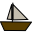
\includegraphics{../gui/data/caravelle}
\end{center}
La Caravelle peut coloniser des îles et déplacer de l'or. Elle doit être
utilisée sur chaque île vierge pour la coloniser.
\begin{itemize}
	\item Coût~: 3 pièces d'or
	\item Déplacement~: 4 cases
\end{itemize}

\subsubsection{Le Galion}
\begin{center}
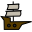
\includegraphics{../gui/data/galion}
\end{center}
Le Galion est un navire de combat. Il peut attaquer une flotte ou une île si
celle-ci se trouve sur la même case que lui.
\begin{itemize}
	\item Coût~: 1 pièce d'or
	\item Déplacement~: 6 cases
\end{itemize}

\subsection{La carte}
La carte est constituée de plusieurs éléments :
\begin{itemize}
	\item La mer~: de grandes étendues d'eau ouvertes à la navigation pour tous\footnote{Pour ou contre la navigation pour tous ?}.
	\item Les îles~: des morceaux de terre sur lesquels vous pouvez construire une
		colonie et construire des navires.
	\item Les volcans~: un certain type d'îles qui rapportent plus d'or que les îles classiques, mais
		trop dangereuses pour y installer un chantier naval.
\end{itemize}

Vous possédez au départ une île, votre point de départ. Vous pouvez coloniser
les autres îles de la carte.
Chaque île rapporte chaque jour un montant fixe d'or.
Deux îles peuvent être «~collées~»~: elles sont toujours considérées comme deux
îles différentes, mais sans bras de mer les séparant.

\subsection{Actions}

\subsubsection{Construction}
Vous pouvez construire sur chaque île des bateaux si vous possédez assez d'or
sur l'île en question. Vous ne pouvez les déplacer qu'au tour suivant.

\subsubsection{Déplacement}
Vous pouvez vous déplacer sur la mer et les îles. Un bateau ne peut
pas être déplacé plusieurs fois par tour, mais chaque bateau peut être déplacé d'autant de
cases qu'il a dans sa portée. À noter que se déplacer en diagonale compte comme deux cases de déplacement.

\subsubsection{Attaque}
Lors d'une attaque sur une case, le vainqueur est celui qui a le plus de galions sur cette case. En cas d'égalité, c'est
l'attaquant qui gagne si on est en mer, et le défenseur si on est sur une
île. Le vainqueur perd autant de galions que le perdant en avait, moins
un. Le perdant perd tout ce qui se trouvait sur la case (galions, caravelles et contrôle de l'île).

Si le combat se déroule sur une île, l'île est attribuée au vainqueur et il
récupère l'or qui s'y trouvait. Si le combat se déroule en mer, l'or contenu
dans les caravelles du perdant est ajouté dans la caravelle du gagnant ayant
l'ID la plus petite\footnote{Fait mystérieux, je vous l'accorde.}. Si le gagnant n'a aucune caravelle, cet or est perdu.

\section{Butin de prise}

\subsection{Score}
Le score de chaque joueur est déterminé à la fin de la partie comme étant son patrimoine total : la
totalité de l'or qu'il possède, plus son nombre de caravelles multiplié par 3, plus son nombre de galions, plus l'or que ses caravelles transportent.

\subsection{Résumé}
Le sujet de la finale de Prologin 2013 est un jeu de stratégie en tour par tour
où chaque joueur contrôle une flotte de bateaux qu'il doit utiliser pour
conquérir les îles de la carte.

Les joueurs vont pour cela coloniser des îles Vierges et attaquer les îles des
autres joueurs, afin d'affirmer leur domination sur l'archipel et ainsi récolter
un maximum d'or et s'armer d'une gigantesque flotte.
